\documentclass{beamer}

% \usepackage{beamerthemesplit} // Activate for custom appearance

\usepackage{graphicx}


\title{{\small INFO 411 presentation on:} \\ \bigskip Callaghan et al. (2002) {\em Streaming-Data Algorithms for
  High-Quality Clustering}} \author{Noel Park, Kat Lilly and Loren
  Kersey} \date{\today}

\begin{document}

\frame{\titlepage}

\section[Outline]{}
\frame{\tableofcontents}

\section{Introduction, Background - Noel's bit}

\frame
{
  \frametitle{Introduction - Data stream model}
  
  Data stream models are mainly preferred when they are based around a large data stream:

  \begin{itemize}
    \item large volume of data is arriving continuously.
    \item unnecessary or impractical to store data in memory.
    \newline
  \end{itemize}

  Data stream models are mainly restricted by:
  \begin{itemize}
    \item in order access to data (as they arrive).
    \item small memory consumption.
    \newline
  \end{itemize}

  This paper by O'Callaghan et al. (2002) describes a streaming
  algorthim that effectively clusters large data streams.

  %NOTES:
  % 
  % dataset -> stored set of data, appropriate for clustering models that query data set again and again.
  % data stream -> approriate model when large volume of data arrives continuously
  % item 1: 
  % item 2: 
  % item 3: random access to memory not allowed.
  % item 4: limited amount of information can be stored.
  % challenge is to perform meaningful computations within these restrictions.
}

\frame
{
  \frametitle{Background - Related Works}
  

  %NOTES:
}

\section{The new algorithm described in this paper - Kat's bit}

\frame
{
  \frametitle{The Clustering Problem}

  The problem this paper focuses on is the following version of the
  clustering problem: 
  
  \begin{itemize}
  \item given an integer {\em k} and a dataset {\em N}, find {\em k}
    cluster centers an assign each {\em n} to the nearest centre
  \item measure the quality of the clustering by the sum of the
    squared distances (SSQ) of the data points to their assigned centers.
  \item Find an optimal or near optimal solution by minimising SSQ.
  \end{itemize}

  The general K-median problem is an NP-hard problem, but there are
  various algorithms for SSQ minimisation that produce near-optimal
  solutions in near-linear time.

  \bigskip
  This paper describes a new such algorithm suitable for streaming
  data.
  
}

\frame
{
  \frametitle{Facility Location Problem}

  Instead of specifying a limit on the value of {\em k}, impose
  a cost for each cluster center (called a `facility' here).

  \bigskip
  The aim now is to minimise both the distance metric and the
  sum of the facility costs,
  \begin{itemize}
  \item so long as a suitable value for the facility cost is
    chosen, an appropriate number of clusters be found.
  \end{itemize}
  \bigskip
  Again this is an NP-hard problem, but several algorithms are
  known that produce near-optimal solutions.

  
}


\frame
{
  \frametitle{STREAM Algorithm}

  The new algorithm described in this paper is called STREAM.

  The deal with arriving data in small chunks - either the data
  arrives that way or they wait until enough data arrives to deal wiht
  it this way.

  They use their new algorithm LSEARCH to cluster each chunk of data.

 

}

\frame
{
  \frametitle{LSEARCH algorithm}

   \begin{itemize}
  \item Once the clustering of each chunk is done, they original data
    is discarded, and only the k cluster centers are stored. Each
    cluster being weighted by the number of sum of the weights of its
    members.

  \item The number of points stored in memory at any given time is
    {\em ik}, where {\em i} is the number of chunks of data processed
    and {\em k} is the number of clusters.

  \item If the number of points in memory becomes too large, at any
    point we can cluster the {\em ik} clusters to reduce the data to
    just {\em k} clusters.
  \end{itemize}

}

\section{Comparison with existing methods - Loren's bit}
\frame
{
  \frametitle{Comparison with other methods}
  To assess the performance of their new clustering and streaming algorithms, O'Callaghan et al. compare them to existing techniques.
  
  \bigskip 
  \begin{itemize}
  \item{LSEARCH performs a similar function to k-means}
  \item{STREAM performs a similar function to BIRCH
    \begin{itemize}
      \item{BIRCH - balanced iterative reducing and clustering using hierarchies - is another streaming algorithm which uses a clustering algorithm as a sub-routine.}
    \end{itemize}
  }
  	     
  \end{itemize}
}

\frame
{
  \frametitle{LSEARCH vs k-means}
  
  \begin{columns}
  
    \begin{column}{0.5\textwidth}
       \begin{itemize}
          \item{Generated 28 small data-sets with between 5 and 16 uniform density spheres}
          \item{For each data-set, calculate SSQ to use as an upper-bound for the optimal SSQ}
          \item{Overlay each data-set with random noise}
          \item{Run LSEARCH and k-means 10 times over each data-set}
      \end{itemize}
    \end{column}
    
    \begin{column}{0.5\textwidth}
        \begin{center}
         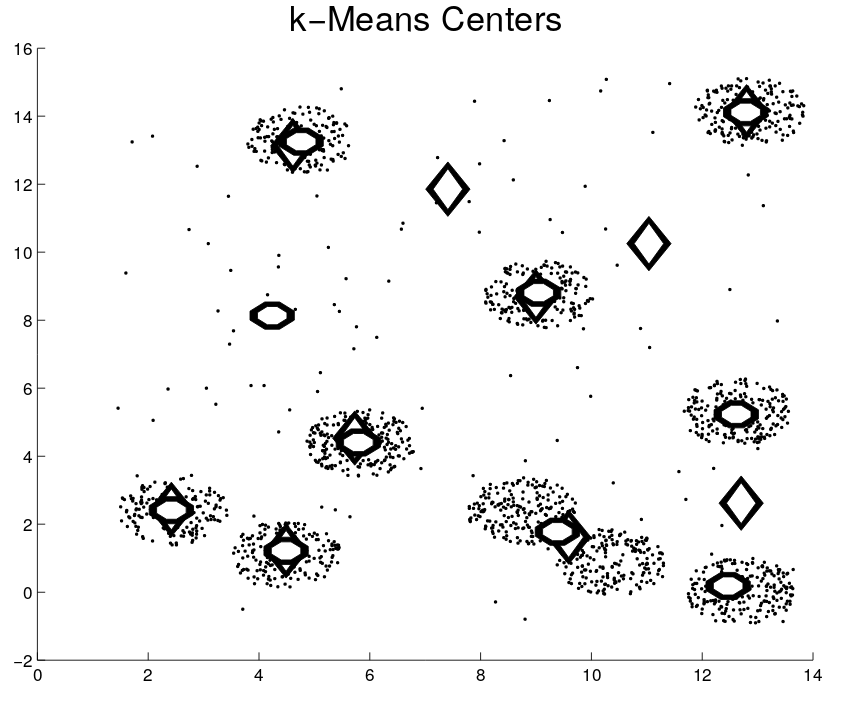
\includegraphics[width=\textwidth]{figures/k-means_clusters.png}      
        \end{center}
    \end{column}
    
  \end{columns}  
}

\frame
{
  \frametitle{LSEARCH vs k-means - results}
  
  \begin{columns}
  
    \begin{column}{0.4\textwidth}
    	  \begin{itemize}
    	  	\item[]{k-means:
    	  	  \begin{itemize}
    	  	    \item{fails to distinguish two close centers}
    	  	    \item{easily distracted by random noise}
    	  	    \item{comparatively high variance in SSQ}
    	  	  \end{itemize}
    	  	}
    	  	\item[]{LSEARCH:
    	  	  \begin{itemize}
    	  	    \item{low variance in SSQ across all data-sets, consistently close to optimal}
    	  	  \end{itemize}
    	  	}
    	  \end{itemize}
    	  
    \end{column}
    
    \begin{column}{0.6\textwidth}
        \begin{center}
         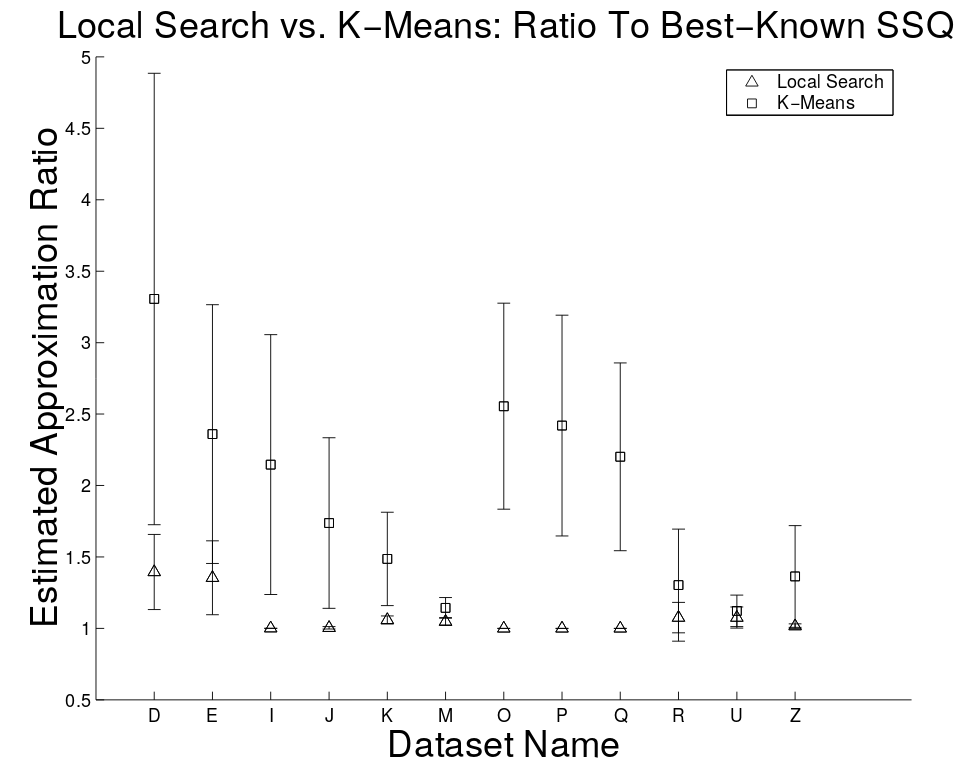
\includegraphics[width=\textwidth]{figures/LSEARCH_vs_k-means.png}      
        \end{center}
    \end{column}
    
  \end{columns}  
}




\frame
{
  \frametitle{STREAM vs BIRCH}
  BIRCH uses a CF-tree to compress a large set of data. The leaves of the CF-tree contain sufficient statistics for a subset of points. A clustering algorithm then clusters the leaf entries. 
  
  Both STREAM and BIRCH repeatedly pre-cluster the data. 
}


\frame[t]{
  \frametitle{References}

  O'Callaghan, L., Mishra, N., Meyerson, A., Guha, S. \& Motwani,
  R. (2002). \textit{Streaming-data algorithms for high-quality
    clustering.} In proceedings of the 18th International Conference
  on Data Engineering. Available from:
  http://ieeexplore.ieee.org/document/994785/.  }
  
\end{document}
